\section{Materials and methods}
\label{sec:framework}
\label{app:campaign}

Read--Answer--Write (RAW) starts with a probe, a simple classifier that reads a finding from the model's image features. We then ask the model about the finding and record its answer. The probe supplies a direction, a way to change the image features so that the probe sees more evidence for the finding. We add that direction to the features and record how the model's answers change. We compare those changes with the effects of directions for other findings and with random and shuffled controls. We use these comparisons to grade how well the model represents and answers each finding, and how selectively an edit controls its answer.

\subsection{Datasets, labels and cohorts}
\label{sec:setup}
\label{app:cf-labels}
\label{app:repro-cohorts}

We used frontal radiographs from NIH ChestX-ray14 and CheXpert Plus. Both datasets label findings from radiology reports.\cite{wang2017chestxray,chambon2024chexpertplus,irvin2019chexpert} We selected frequent findings with enough positive cases. Both datasets included effusion, atelectasis, pneumothorax, and cardiomegaly. We also included mass and nodule on NIH and consolidation and edema on CheXpert Plus. The natural-image control used COCO labels for person, dog, car, chair, bottle, and bicycle.\cite{lin2014coco} We excluded uncertain or blank labels when fitting probes or scoring agreement with labels. We included those images when measuring how edits changed the model's answers.

All models used the same image lists for training, calibration, and testing. We fitted probes on the training list. We graded reading and answering on the calibration list and measured edits on the test list. The lists shared no patients or COCO images. NIH training used \cfCohortNihTrainRows{} studies from \cfCohortNihTrainUnits{} patients. Of these, \cfCohortNihTrainMulti{} contributed multiple studies, with up to \cfCohortNihTrainMax{} from one patient. All other lists used one image per patient or COCO image. CheXpert Plus and COCO each supplied \cfCohortChexTrainRows{} training images. Each dataset supplied \cfCohortNihCalibrationRows{} calibration and \cfCohortNihTestRows{} test images. Separate cohorts supplied the NIH replication images and \cfValidRows{} CheXpert films with radiologist consensus labels.\cite{irvin2019chexpert}

We selected smaller COCO objects to test the role of question difficulty. An eligible category needed at least as many positive training examples as the smallest original category. They needed at least \jnMinClassSupport{} positives in each of the calibration and test cohorts. Their mean relative area had to be below the original categories' median. We took the \jnCoreConceptCount{} categories with the most calibration positives, breaking ties by smaller area and then category identifier.

\subsection{Models and image features}
\label{app:cf-grid}

We evaluated \cfCheckpoints{} trained versions of models, called checkpoints, from \cfFamiliesWord{} general-purpose and medical families (Table~\ref{tab:cf-models}). We call each checkpoint--dataset pair a block. Each finding or object within a block is a cell. We scored about \jnScoredAnswersMillions{} million answers across \cfBlocks{} blocks and \cfCells{} cells.

The vision tower is the part of the model that encodes the image. It represents the image as lists of numbers called visual tokens. The connector prepares those tokens for the language model. We call the connector and language model together the reader. We edited the last image features that the tower sent to the connector. We also edited the connector's output to test how the language model responded when it received the edit directly. The location and selection of tokens for each model appear in Section~\ref{app:repro-sites}.

LLaVA uses CLIP,\cite{radford2021clip} which HuatuoGPT-Vision-7B retains after medical tuning. Gemma~3 uses SigLIP,\cite{zhai2023siglip} MedGemma uses medically tuned SigLIP,\cite{sellergren2025medgemma} and Qwen3-VL uses a SigLIP~2 design.\cite{tschannen2025siglip2} The chest-trained towers are XraySigLIP in CheXagent-2-3B, EVA-CLIP in CheXagent-8B, and BiomedCLIP-CXR in LLaVA-Rad-7B.\cite{chen2024chexagent,sun2023evaclip,zhang2025biomedclip,zambranochaves2025llavarad}

\begin{table*}[pos=tp]
\centering
\setlength{\tabcolsep}{3pt}
% terracotta = positive / high, blue = negative / low, sage = magnitude of Read and Ans; darker = larger magnitude
\definecolor{cfSage1}{HTML}{ECF3EF}
\definecolor{cfSage2}{HTML}{D5E5DB}
\definecolor{cfSage3}{HTML}{B9D4C3}
\definecolor{cfSage4}{HTML}{9EC3AC}
\definecolor{cfSlate1}{HTML}{EAF0F6}
\definecolor{cfSlate2}{HTML}{D0DDEA}
\definecolor{cfSlate3}{HTML}{B1C7DD}
\definecolor{cfSlate4}{HTML}{94B2D0}
\definecolor{cfTerra1}{HTML}{F7ECEA}
\definecolor{cfTerra2}{HTML}{EED5D1}
\definecolor{cfTerra3}{HTML}{E2B8B2}
\definecolor{cfTerra4}{HTML}{D79E95}
\definecolor{cfOat1}{HTML}{F4EFE6}
\definecolor{cfOat2}{HTML}{E8DDC8}
\definecolor{cfGrey}{HTML}{E4E1DC}

\caption{\textbf{Checkpoints and families.} Checkpoint rows give the vision tower, visual tokens passed to the connector per image, input size, and eligible templates. Bold family rows give mean selectivity and clean-answer AUROC over clinical cells, then the owned clinical and COCO cells, shaded by owned share.}
\label{tab:cf-models}
\fitwidth{%
\cftabsize
\begin{tabular}{lllll@{\hspace{8pt}}rrrr}
\toprule
\multirow{2}{*}{Checkpoint} & \multirow{2}{*}{Vision tower} & \multirow{2}{*}{Tokens} & \multirow{2}{*}{Image} & \multirow{2}{*}{Templates} & \multirow{2}{*}{$\bar S$} & \multirow{2}{*}{$\overline{\mathrm{AUROC}}$} & \multicolumn{2}{c}{owned cells}\\
\cmidrule(lr){8-9}
&  &  &  &  &  &  & \multicolumn{1}{c}{clinical} & \multicolumn{1}{c}{COCO}\\
\midrule
\multicolumn{5}{l}{\textbf{Qwen2.5-VL}\cite{bai2025qwen25vl}} & 0.132 & 0.635 & \cellcolor{cfTerra2}5/48 & \cellcolor{cfTerra4}24/24 \\
\quad Qwen2.5-VL-3B & native ViT 675M & 576$\to$144 & $336^2$ & IYWYIAWA & & & & \\
\quad Qwen2.5-VL-7B & native ViT 675M & 576$\to$144 & $336^2$ & all & & & & \\
\quad Qwen2.5-VL-32B & native ViT 675M & 576$\to$144 & $336^2$ & all & & & & \\
\quad Qwen2.5-VL-72B & native ViT 675M & 576$\to$144 & $336^2$ & all & & & & \\
\midrule
\multicolumn{5}{l}{\textbf{Qwen3-VL}\cite{qwen2025qwen3vl}} & 0.137 & 0.735 & \cellcolor{cfTerra3}6/36 & \cellcolor{cfTerra4}18/18 \\
\quad Qwen3-VL-4B & SigLIP2-based & $\leq$1024 & $\leq 512^2$ & all & & & & \\
\quad Qwen3-VL-8B & SigLIP2-based & $\leq$1024 & $\leq 512^2$ & all & & & & \\
\quad Qwen3-VL-32B & SigLIP2-based & $\leq$1024 & $\leq 512^2$ & all & & & & \\
\midrule
\multicolumn{5}{l}{\textbf{InternVL3.5}\cite{wang2025internvl35}} & 0.125 & 0.807 & \cellcolor{cfTerra3}6/36 & \cellcolor{cfTerra4}18/18 \\
\quad InternVL3.5-8B & InternViT-300M & 1024 & $448^2$ & all & & & & \\
\quad InternVL3.5-14B & InternViT-300M & 1024 & $448^2$ & all & & & & \\
\quad InternVL3.5-38B & InternViT-6B & 1024 & $448^2$ & all & & & & \\
\midrule
\multicolumn{5}{l}{\textbf{Gemma 3}\cite{gemma2025gemma3}} & 0.124 & 0.564 & \cellcolor{cfTerra2}4/36 & \cellcolor{cfTerra4}17/18 \\
\quad Gemma 3 4B & SigLIP-So400m & 4096 & $896^2$ & all & & & & \\
\quad Gemma 3 12B & SigLIP-So400m & 4096 & $896^2$ & all & & & & \\
\quad Gemma 3 27B & SigLIP-So400m & 4096 & $896^2$ & all & & & & \\
\midrule
\multicolumn{5}{l}{\textbf{MedGemma} (medical)\cite{sellergren2025medgemma}} & 0.164 & 0.835 & \cellcolor{cfTerra2}2/24 & \cellcolor{cfTerra3}10/12 \\
\quad MedGemma 4B & MedSigLIP & 4096 & $896^2$ & all & & & & \\
\quad MedGemma 27B & MedSigLIP & 4096 & $896^2$ & all & & & & \\
\midrule
\multicolumn{5}{l}{\textbf{Lingshu} (medical)\cite{lasa2025lingshu}} & 0.142 & 0.820 & \cellcolor{cfTerra4}12/24 & \cellcolor{cfTerra4}12/12 \\
\quad Lingshu 7B & Qwen2.5-VL ViT & 576$\to$144 & $336^2$ & all & & & & \\
\quad Lingshu 32B & Qwen2.5-VL ViT & 576$\to$144 & $336^2$ & all & & & & \\
\midrule
\multicolumn{5}{l}{\textbf{LLaVA-1.5}\cite{liu2024improved}} & 0.124 & 0.516 & \cellcolor{cfTerra1}0/24 & \cellcolor{cfTerra3}8/12 \\
\quad LLaVA-1.5-7B & CLIP ViT-L/14-336 & 576 & $336^2$ & IYWY & & & & \\
\quad LLaVA-1.5-13B & CLIP ViT-L/14-336 & 576 & $336^2$ & IYWYIAWA & & & & \\
\midrule
\multicolumn{5}{l}{\textbf{LLaVA-Med} (medical)\cite{li2023llavamed}} & 0.136 & 0.560 & \cellcolor{cfTerra2}1/12 & \cellcolor{cfTerra2}1/6 \\
\quad LLaVA-Med 1.5 7B & CLIP ViT-L/14-336 & 576 & $336^2$ & IYWY & & & & \\
\midrule
\multicolumn{5}{l}{\textbf{Llama 3.2 Vision}\cite{meta2024llama32vision}} & 0.119 & 0.688 & \cellcolor{cfTerra1}0/12 & \cellcolor{cfTerra2}1/6 \\
\quad Llama 3.2 Vision 11B & ViT-H/14 & 1601 & $560^2$ & IBWB & & & & \\
\midrule
\multicolumn{5}{l}{\textbf{CheXagent} (medical)\cite{chen2024chexagent}} & 0.180 & 0.857 & \cellcolor{cfTerra3}7/24 & \cellcolor{cfTerra2}2/12 \\
\quad CheXagent-2-3B & XraySigLIP ViT-L/16 & 1024 & $512^2$ & IYWYIAWA & & & & \\
\quad CheXagent-8B & EVA-CLIP ViT 1.4B & 1025$\to$128 & $448^2$ & IYWYIAWA & & & & \\
\midrule
\multicolumn{5}{l}{\textbf{LLaVA-Rad} (medical)\cite{zambranochaves2025llavarad}} & 0.209 & 0.793 & \cellcolor{cfTerra1}0/12 & \cellcolor{cfTerra1}0/6 \\
\quad LLaVA-Rad-7B & BiomedCLIP-CXR-518 & 1369 & $518^2$ & IYWY & & & & \\
\midrule
\multicolumn{5}{l}{\textbf{HuatuoGPT-Vision} (medical)\cite{chen2024huatuogptvision}} & 0.136 & 0.746 & \cellcolor{cfTerra2}1/12 & \cellcolor{cfTerra4}6/6 \\
\quad HuatuoGPT-Vision-7B & CLIP ViT-L/14-336 & 576 & $336^2$ & all & & & & \\
\bottomrule
\end{tabular}}
\end{table*}


\subsection{Reading and writing findings}
\label{sec:site}

\begin{figure*}[pos=tp]
    \centering
    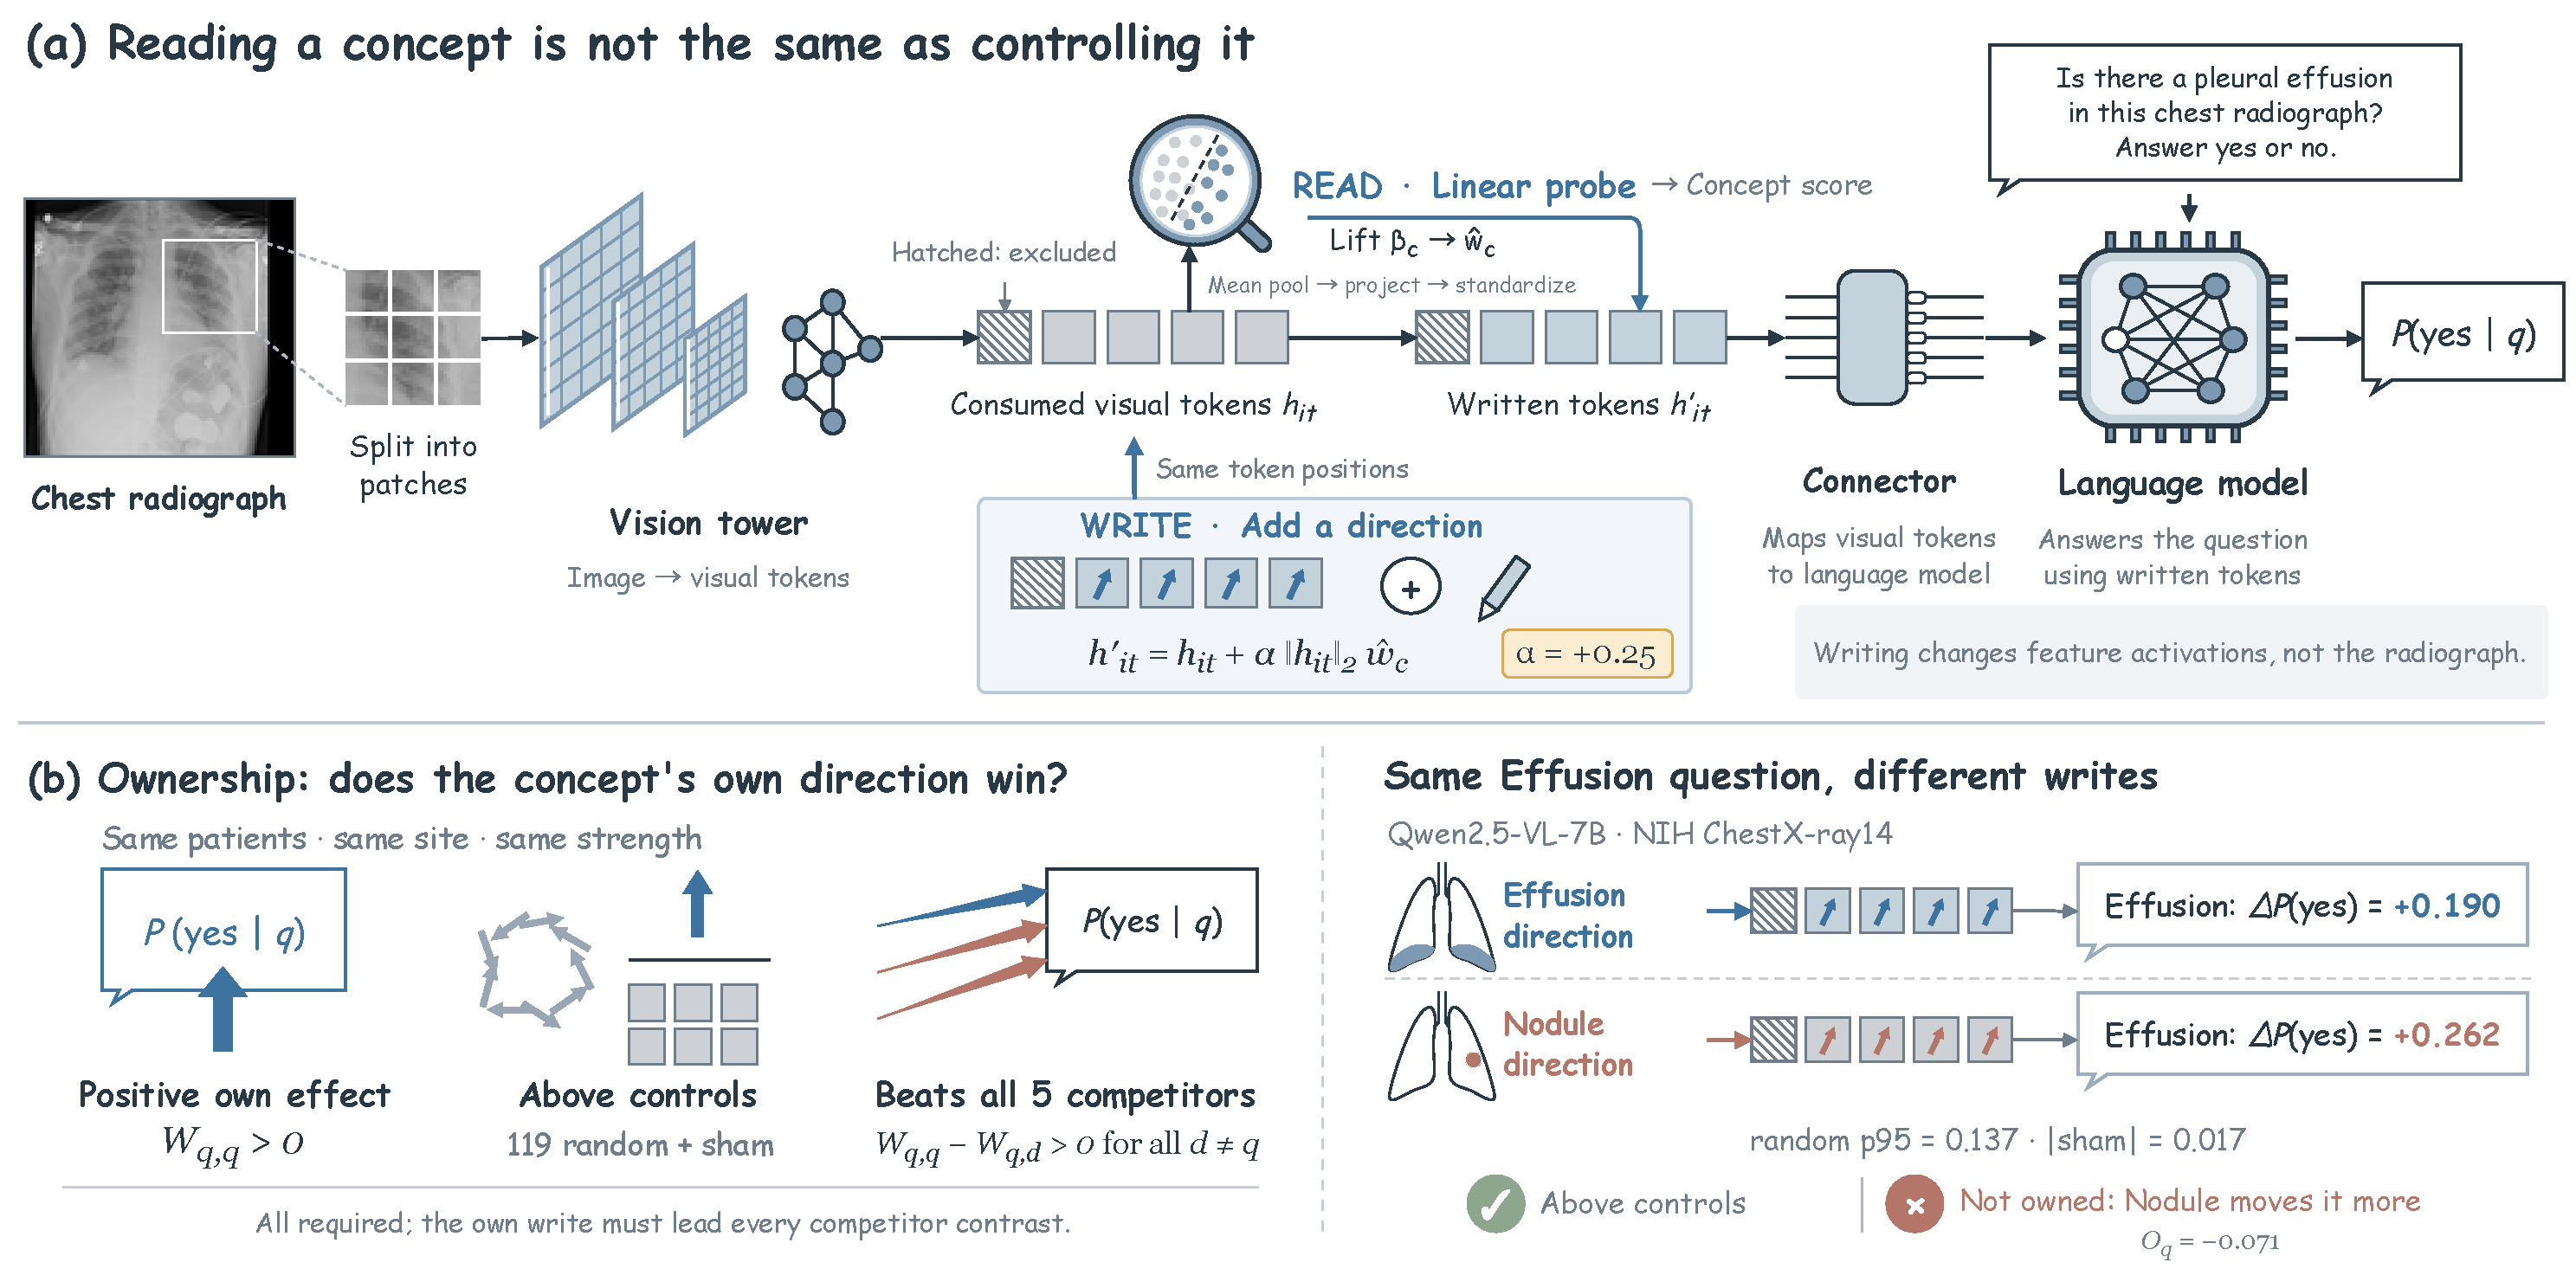
\includegraphics[width=\linewidth]{figures/fig1_framework.pdf}
    \caption{\textbf{Reading and writing at the selected vision layer.} (a) The probe reads the visual tokens that receive the write. Hatching marks token positions the connector excludes. (b) On NIH ChestX-ray14, the nodule write raises Qwen2.5-VL-7B's effusion answer more than the effusion write does.}
    \label{fig:framework}
\end{figure*}

For each image, we averaged the tokens from the selected layer. We reduced the number of features and put them on a common scale using the training images. We fitted a logistic regression probe to predict whether each finding was present. The \emph{label direction} is the change in the original image features that most increases the probe score per unit of change (Eq.~\ref{eq:lift}).

A write adds the direction to the tokens the probe read (Fig.~\ref{fig:framework}). To compare edits across models, we set the \emph{steering strength} relative to each token's length. The main edit used a fraction of \jnPrimaryStrength{} to move toward higher probe scores. We also tested other strengths (Section~\ref{sec:write-implementation}).

\subsection{Controls for reading and writing}
\label{sec:directions}

We measured probe performance with the area under the receiver operating characteristic curve (AUROC). It estimates the chance that a positive example scores higher than a negative example, with half credit for ties. We compared the probe's AUROC with that of probes trained on randomly assigned labels. Images of the same type shared a random label. On chest radiographs we grouped images by projection, recorded sex, and age decade. On COCO we used aspect ratio and area. The concept probe's AUROC minus the mean AUROC of valid random-label probes is its \emph{selectivity}, denoted by $S$ (Eq.~\ref{eq:selectivity}).

A \emph{competitor} is a direction fitted to another finding or object. We also drew \jnRandomDirections{} random directions. A \emph{sham} shuffles the values of the target direction. All controls used the same strength and images as the target direction.

\subsection{Questions and scoring}
\label{app:protocol}

The questions used \emph{is there} (I) or \emph{does the image show} (W). Both wordings used yes/no (Y) and two letter mappings (A-present and B-present). The primary prompt was IY. When yes/no failed the answer mapping check, we graded a valid letter-coded prompt (Section~\ref{app:cf-gates}).

For each question we measured the model's support for yes relative to no at the first answer position. We write this score as $P(\mathrm{yes})$. The \emph{clean answer} is the score before an edit. We also used the \emph{answer margin}, the difference between the log probabilities of yes and no before conversion to a score (Section~\ref{sec:scoring-implementation}). Tables~\ref{tab:key-terms} and \ref{tab:notation} summarize the terms and symbols.

\begin{table}[pos=b]
\centering
\caption{\textbf{Key terms.} Definitions for the RAW evaluation.}
\label{tab:key-terms}
\fitwidth{%
\cftabsize
\begin{tabular}{@{}lp{0.70\columnwidth}@{}}
\toprule
Term & Definition \\
\midrule
Probe & Classifier fitted to the model's image features. \\
Direction & Vector specifying how features change. \\
Write & Addition of a direction to the features. \\
Reader & Connector and language model. \\
Competitor & Direction fitted for another labeled concept. \\
Sham & Control made by shuffling a direction's coordinates. \\
Cell & One checkpoint and one concept on a dataset. \\
Block & One checkpoint evaluated on one dataset. \\
\bottomrule
\end{tabular}}
\end{table}

\begin{table*}[pos=tp]
\centering
\caption{\textbf{Notation used in the study.} Symbols for features, answers, and effects of edits.}
\label{tab:notation}
\fitwidth{%
\cftabsize
\begin{tabular}{@{}lp{0.80\linewidth}@{}}
\toprule
Symbol & Definition \\
\midrule
$c$, $q$, $d$ & Concept, question about a concept, and direction fitted for a concept. \\
$\hvec_{it}$, $\hvec_i$ & Visual token $t$ of image $i$ and the mean of its selected tokens. \\
$D$, $R$, $\boldsymbol s$, $\boldsymbol\beta_c$ & Vision feature dimension, Gaussian projection, training feature scales, and probe coefficients. \\
$\hat\wvec_c$, $a_q$ & Directions fitted to labels (Eq.~\ref{eq:lift}) and to clean answers (Eq.~\ref{eq:answer-direction}). \\
$\alpha$, $S$ & Signed edit strength relative to token length and probe selectivity (Eq.~\ref{eq:selectivity}). \\
$W_{q,d}$ & Mean change in question $q$'s score under direction $d$. \\
$O_q$, $C_d$ & Row and column margins (Eqs.~\ref{eq:margin} and \ref{eq:column-margin}). \\
$O_q^m$ & Row margin calculated from changes in the log-probability difference for yes versus no. \\
$\kappa_d$ & Signed own effect divided by total absolute change (Eq.~\ref{eq:column-selectivity}). \\
$F_{q,d}$ & Mean positive change over checkpoints, shown by band width in Fig.~\ref{fig:write-flow}. \\
$\cos_\Sigma$ & Cosine weighted by training-feature covariance $\Sigma$ (Eq.~\ref{eq:whitened-cos}). \\
\bottomrule
\end{tabular}}
\end{table*}

\subsection{Ownership and direction specificity}
\label{sec:ownership}

The write matrix has one row per question and one column per direction. Entry $W_{q,d}$ is the mean change to answer $q$ when we add direction $d$ on the same test images. The diagonal entry $W_{q,q}$ is the \emph{own write}. It meets the steering reference if the increase exceeds the ninety-fifth percentile of random effects and the absolute sham effect.

\emph{Ownership} asks which direction raises a given answer the most. The row margin $O_q$ subtracts the largest competing effect from the own write.
\begin{equation}
O_q=W_{q,q}-\max_{d\ne q}W_{q,d}.
\label{eq:margin}
\end{equation}
A cell is owned when it meets the steering reference and this margin is positive.

\emph{Direction specificity} asks which answer changes most under a given direction. The column margin $C_d$ subtracts the largest absolute change on any other answer from the own write.
\begin{equation}
C_d=W_{d,d}-\max_{q\ne d}\lvert W_{q,d}\rvert.
\label{eq:column-margin}
\end{equation}
A cell is specific when it meets the reference and this margin is positive. A large decrease in another answer counts against specificity. We report total absolute change in other answers relative to the own write. \emph{Column selectivity} $\kappa_d$ measures the share attributable to the signed own write.
\begin{equation}
\kappa_d=\frac{W_{d,d}}{\sum_q\lvert W_{q,d}\rvert}.
\label{eq:column-selectivity}
\end{equation}
It equals one if the edit raises only its own answer and leaves the others unchanged.

\subsection{Decision rules and supporting analyses}
\label{sec:grades}

\begin{table}[pos=t]
\centering
\caption{\textbf{RAW grades.} Reading and answering use calibration data. Intervention criteria use the test cohort.}
\label{tab:grades}
\fitwidth{%
\cftabsize
\begin{tabular}{@{}lp{0.62\columnwidth}@{}}
\toprule
Grade & Criterion \\
\midrule
Readable & Probe selectivity $S>0$ \\
Answerable & Clean-answer AUROC above chance \\
Owned & Steering reference met and $O_q>0$ \\
Specific & Steering reference met and $C_d>0$ \\
Owned and specific & Steering reference met, $O_q>0$ and $C_d>0$ \\
\bottomrule
\end{tabular}}
\end{table}

To grade readability or answerability, we required at least \jnMinClassSupport{} known positives and \jnMinClassSupport{} known negatives in the calibration group. Readability also required a valid AUROC for the finding probe and at least \jnMinValidControls{} valid control AUROCs. Table~\ref{tab:grades} gives the criteria. To assess sensitivity to the choice of competitors, we repeated the comparison for every subset of a given size and averaged the owned counts.

We compared alternative directions and tested edits concentrated on high-scoring tokens. We regraded changes on the answer-margin scale, using $O_q^m$ for its row margin. We repeated grading on images with a clean yes score between \jnSaturationLow{} and \jnSaturationHigh{}, and grouped results by clean answer and label. We checked the grades against radiologist consensus and applied directions fitted to those labels to the main test cohort. For comparison, we fitted directions to report labels from the same films, size-matched training subsets, and the full training set.

\label{app:cf-difficulty}
We graded the smaller COCO objects on the same checkpoints and images as the original objects. We pooled both COCO sets and grouped cells by clean-answer AUROC at \cfStratEdges{}. We also compared cells at minimum AUROCs of \jnCsAurocLower{} and \jnCsAurocHigher{}, where the domains overlapped more. A logistic model predicted ownership from image domain, AUROC, and probe selectivity. For each cell we predicted ownership under both domains at its observed AUROC and selectivity. We averaged the differences between those predictions. For the adjusted results and highest AUROC group, we estimated standard deviations from \jnBootstrapResamples{} resamples of whole checkpoints with replacement.

We also graded directions for projection (anteroposterior or portable versus posteroanterior), recorded sex, and age at least \jnAttributeAgeCutoff{} years. The attributes and findings competed in \cfAttrRefBlocks{} blocks under the same controls. Calibration tried \cfAttrqPhrasings{} wordings per attribute. We compared all cells, answerable cells, and cells matched within \cfAttrPairWindow{} clean-answer AUROC in the same block.

To test the reader's role, we paired the Gemma~3 4B and MedGemma 4B towers with both readers. Directions stayed with the towers. We also gave readers from shared-tower checkpoints the same stored features and edits (Section~\ref{app:cf-crossed-reader}).

We fitted an \emph{answer direction} to unedited answers. We compared its alignment and agreement with labels against the label direction. We also tested negated questions and choices between the finding and its strongest competitor, in both orders. A further test scored the finding word in a report continuation (Section~\ref{sec:scoring-implementation}).

\subsection{Registration and reproducibility}
\label{app:repro}
\label{app:repro-protocol}

We registered the layers, settings, controls, prompts, and rules before scoring. Dated amendments preceded the additional analyses, including category selection and difficulty comparisons. Rankings, changes across answers, and individual examples describe the completed runs. The release includes code, adapters, protocol, cohort lists and seeds, directions, image-level results, scorecards, and prompts.

\subsubsection{Registered NIH replication and prompt experiments}
\label{app:seed}

The NIH experiments used LLaVA-1.5-7B for effusion and edema and Qwen2.5-VL-7B for effusion.\cite{liu2024improved,bai2025qwen25vl} We assigned patients to separate training, validation, and test groups by hashing their identifiers. Training used \jnReplicationTrainingRows{} images. The held-out group included \jnReplicationTestRows{} images from \jnReplicationTestPatients{} patients. We verified that the write reached the answer scores and that zero strength reproduced the clean answer. Selectivity used \jnLabelControlCount{} random-label maps over \jnReplicationLabelTypes{} image types.

We tested the initial writes across several strengths on \jnReplicationInitialRows{} images (Section~\ref{sec:write-implementation}). Controls included \jnLabelControlCount{} random directions, the sham, and the fixed competitors. For the strengths in $\mathcal A=\jnReplicationControlStrengths$, we picked the strength $\alpha_c^\star$ that gave the largest change in the intended direction. Here $\Delta_c(\alpha)$ is the mean change from the clean score for concept $c$ at strength $\alpha$, and $\Delta_c^\star$ is the selected signed change.
\begin{equation}
\begin{aligned}
\alpha_c^\star &=
  \operatorname*{arg\,max}_{\alpha\in\mathcal A}
  \operatorname{sign}(\alpha)\Delta_c(\alpha),\\
\Delta_c^\star &=\operatorname{sign}(\alpha_c^\star)
                 \Delta_c(\alpha_c^\star).
\end{aligned}
\label{eq:seed-rule}
\end{equation}
We compared the selected change with the largest absolute sham effect across controlled strengths and the ninety-fifth percentile of signed random effects at the selected strength. We described how steadily the scores moved over $\jnStrengthSweepBounds$.

At the primary strength we tested one image from each of \jnReplicationEffusionRows{} new patients selected by label-blind hash. With \jnLabelControlCount{} random directions, a sham, and clinical competitors, this gave \jnReplicationConfigurations{} conditions and \jnReplicationOutcomeCount{} image-level outcomes. The own write had to exceed the random cutoff, sham effect, and competitors. We then tested all findings in \jnReplicationMatrixRows{} new patients using the largest random effect as the cutoff. We measured each direction's mean signed effect on other answers and its excess over their own writes.

The letter-mapping test used \jnReplicationPromptRows{} patients and an equally sized, distinct calibration group. Eligibility required above-chance AUROC under both mappings and \jnMinClassSupport{} patients per class. Edits at $\jnReplicationPromptStrengths$ used \jnLabelControlCount{} random directions and a sham. The mass confirmation used both wordings and all formats in \jnReplicationMassRows{} further patients. The primary write had to beat \jnLabelControlCount{} clinical comparisons, the largest of \jnRandomDirections{} random effects, and the absolute sham effect in all letter conditions or both yes/no conditions (Section~\ref{app:seed-results}).

\subsection{Implementation details}
\label{sec:implementation}

\subsubsection{Vision layers and token selection}
\label{app:repro-sites}
\label{app:repro-mask}

Models ran in bfloat16 with their native processors and fixed resolutions. Processor outputs identified the \cfTokensMin{} to \cfTokensMax{} tokens selected per image.

\begin{itemize}[leftmargin=*,itemsep=1pt,topsep=2pt]
\item Qwen2.5-VL and Lingshu used the last of \jnQwenVisionDepth{} blocks. Qwen3-VL used the last of \jnQwenThreeShallowDepth{} at 4B or \jnQwenThreeDeepDepth{} at 8B and 32B. The patch grid identified each image's contiguous span. The connector merged $\jnPatchGroupSide\times\jnPatchGroupSide$ patches. Earlier DeepStack branches bypassed the edit.
\item Gemma~3 and MedGemma used all normalized patches from the last of \jnSiglipDepth{} SigLIP layers. InternVL3.5 used the last of \jnInternVlShallowDepth{} InternViT layers at 8B and 14B, or \jnInternVlDeepDepth{} at 38B. Its final normalization was an identity. We kept patch tokens from the single tile and excluded its image-summary token (CLS). Patch counts had to match image placeholders.
\item LLaVA-1.5 and LLaVA-Med used the penultimate of \jnClipDepth{} CLIP layers and excluded CLS. Llama~3.2 Vision used the last of \jnLlamaGlobalDepth{} global layers. Its \jnLlamaLocalBranches{} intermediate local inputs bypassed the edit. We kept CLS and the patches of the real tile and excluded its \jnLlamaPaddingTokens{} padding tokens and the \jnLlamaPaddingTiles{} padded tiles.
\end{itemize}

We rejected incomplete spans, mask mismatches, empty images, and repeated calls to the layer in one pass. Records identify the layer, feature dimension, connector, and bypassed branches.

\subsubsection{Probe fitting and control generation}
\label{app:repro-probe}
\label{app:repro-controls}

For image $i$, $\hvec_i$ is its mean selected token vector. Projection matrix $R$ has $D$ original feature rows and $m=\cfAltdirdGramDim$ projected columns. PCG64 with seed zero drew independent standard normal entries. We divided by $\sqrt{m}$ and stored in single precision. We centered features at their training means and scaled by their standard deviations, floored at $\jnScaleFloor$. The $\ell_2$-regularized fit used unweighted classes, inverse penalty $C=1$, and up to \jnProbeMaxIterations{} L-BFGS iterations. Refits resampled whole patients or images with replacement and refitted scales and probes with the same projection and control seeds.

To express the fitted direction in the original features, we divide the probe coefficients $\boldsymbol\beta_c$ for finding $c$ by the feature scales $\boldsymbol s$. We map the result back with $R$ to give $\boldsymbol g_c$, then normalize it to unit length to obtain $\hat\wvec_c$.
\begin{equation}
\begin{aligned}
\boldsymbol g_c &= R\,\mathrm{diag}(\boldsymbol s)^{-1}\boldsymbol\beta_c,\\
\hat\wvec_c &= \boldsymbol g_c/\lVert\boldsymbol g_c\rVert_2.
\end{aligned}
\label{eq:lift}
\end{equation}

For the \jnLabelControlCount{} random-label probes we used successive PCG64 seeds starting at zero. We drew equiprobable binary labels for image types in sorted order. If all types received the same label, we flipped the first. We fitted the controls using the same known-label rows and settings as the finding probe. Fitting controls required at least \jnMinControlTypes{} types per block. With labels $y$, probe scores $r$, and $K$ valid controls, selectivity is
\begin{equation}
S=\operatorname{AUROC}(y,r)-
\frac{1}{K}\sum_{k=1}^{K}\operatorname{AUROC}
             (y_k^{\mathrm{ctrl}},r_k^{\mathrm{ctrl}}).
\label{eq:selectivity}
\end{equation}
The subscript $k$ identifies the control and the superscript $\mathrm{ctrl}$ distinguishes its labels and scores.

For the write controls, PCG64 with seed zero drew Gaussian vectors. We normalized each vector to unit length and shared the draws across questions within a block. The same generator produced one coordinate permutation per label direction in protocol order for the shams.

\subsubsection{Writes and alternative directions}
\label{sec:write-implementation}

For token $t$ of image $i$, $\hvec_{it}$ is the original feature vector and $\hvec'_{it}$ is the edited vector. We add the unit direction for finding $c$ after scaling it by the token length and signed steering strength $\alpha$.
\begin{equation}
\hvec'_{it}=\hvec_{it}+\alpha\lVert\hvec_{it}\rVert_2\,\hat\wvec_c.
\label{eq:intervention}
\end{equation}
The main write used $\alpha=\jnPrimaryStrength$. The sweep also tested $\alpha\in\jnOtherStrengths$. The NIH replication used
\[\alpha\in\jnReplicationStrengths.\]

We compared the probe direction with the difference between positive and negative feature means and the activation pattern associated with the probe weights (Haufe pattern).\cite{haufe2014interpretation} Other variants projected the probe away from the competing directions or refitted it after removing the linear contribution of the competing labels. For a direct change $\boldsymbol u$ in the projected and scaled features, we used the shortest corresponding vector in the original features, up to scale.
\begin{equation}
\begin{aligned}
\hat\wvec &\propto R(R^{\top}R)^{-1}
             \mathrm{diag}(\boldsymbol s)\,\boldsymbol u,\\
R^\top\hat\wvec &\propto \mathrm{diag}(\boldsymbol s)\,\boldsymbol u .
\end{aligned}
\label{eq:displacement-lift}
\end{equation}
This conversion differs from the coefficient conversion because $R^\top R$ is not proportional to the identity. The matrix $R^\top R/D$ had full rank $m$ in the \cfAltdirdBlocks{} blocks tested. Its eigenvalues ranged from $\cfAltdirdEigMin$ to $\cfAltdirdEigMax$. Its condition numbers ranged from \cfAltdirdCondMin{} to \cfAltdirdCondMax{}.

We also varied the write across tokens. Each weight $\omega_t$ depends on the token's probe score $z_t$. For $n_{\mathrm{tok}}$ selected tokens, the weights average one. One variant weighted scores by their exponentials (softmax). Another wrote only to the highest-scoring quarter.
\begin{equation}
\begin{aligned}
\hvec'_{it}&=\hvec_{it}+\alpha\omega_t\lVert\hvec_{it}\rVert_2\,\hat\wvec_c,\\
\omega_t^{\mathrm{softmax}}
  &=n_{\mathrm{tok}}e^{z_t}\big/\sum_{t'}e^{z_{t'}},\\
\omega_t^{\mathrm{quarter}}
  &=4\,\mathbf 1[\,z_t\in\text{top quarter}\,].
\end{aligned}
\label{eq:token-weights}
\end{equation}
Here $t'$ ranges over selected tokens and $\mathbf 1$ is one for selected high-scoring tokens and zero otherwise. The softmax kept the sum of weights fixed. The top-quarter variant doubled their Euclidean norm. Extended comparisons added directions for labels with at least \jnMinExtendedClassSupport{} known positives and negatives. These were consolidation, edema, and infiltration on NIH, and enlarged cardiomediastinum, fracture, lung lesion, lung opacity, pneumonia, and support devices on CheXpert Plus.

\subsubsection{Acceptance checks and coverage}
\label{sec:gates}
\label{app:cf-gates}
\label{app:cf-coverage}

We used \cfCohortNihPreflightRows{} images at both sites. Checks covered repeatability (A), zero-strength identity (B), and whether the first concept's primary write changed downstream scores within the token mask (C). We compared batched and single-image passes (D) and tested answer mappings without images (E). We checked throughput (F) and recomputed scores at single precision (G). Each question used fixed image groups across conditions. Eligible prompts passed the mapping check. All \cfWriteBlocks{} completed blocks passed A--C, and single-precision differences were below \cfGateFpMax{}. We rescored the first \jnPrecisionRows{} test rows singly at single precision.

The \cfCoveragePlannedWord{} planned components were the core write matrix and calibration, additional prompts, the strength sweep, probe refits, and writes and calibration at the connector output. All \cfBlocks{} blocks completed the core matrix and calibration. Of these, \cfCoverageBlocksAllSeven{} completed all components. The Qwen2.5-VL-72B CheXpert Plus block lacked the extra prompts and connector tests. A successful probe with an ineligible or incomplete matrix contributed only readability. Scorecards retain the range over $\jnStrengthSweepBounds$, refit standard deviations, connector-output grades, and prompt comparisons. The study used about \jnEvaluationComputeHours{} A100 GPU-hours. A chest block from a model with seven billion parameters took about \jnChestBlockHours{} hours.

\subsubsection{Reader swaps and feature replay}
\label{app:cf-crossed-reader}

In the crossed experiment, the swapped tower matched \cfSwapTensors{} donor weight arrays exactly. The \cfSwapOutside{} arrays outside the tower were unchanged. All combinations used the same \cfSwapRows{} test images, primary strength and prompt, and the controls for the installed tower. Let $Y_q(g/h)$ be the measurement for question $q$ with tower $g$ and reader $h$. The model identifiers $\mathrm G$ and $\mathrm M$ denote Gemma~3 and MedGemma.
\begin{equation}
\begin{aligned}
\delta_{\text{reader}}&=\tfrac{1}{12}\sum_{g,q}
  \lvert Y_q(g/\mathrm G)-Y_q(g/\mathrm M)\rvert,\\
\delta_{\text{tower}}&=\tfrac{1}{12}\sum_{h,q}
  \lvert Y_q(\mathrm G/h)-Y_q(\mathrm M/h)\rvert.
\end{aligned}
\label{eq:crossover}
\end{equation}
The two effects average absolute changes after replacing either the reader or the tower. Measurements were the own write $W_{q,q}$, the row margin $O_q$, and the margin over the largest competing, random-cutoff, or absolute sham effect, denoted by $M_q$. For the replay, we stored the selected tokens from one checkpoint and used them in place of both checkpoints' own features. We first measured how much the stored and original tokens differed. Replaying a checkpoint's own tokens checked the substitution path.

\subsubsection{Answer scores, answer directions, and other response formats}
\label{sec:scoring-implementation}

For each answer we used the highest log probability among its valid single-token forms, including case and leading spaces. Let $\ell_{\mathrm{yes}}$ and $\ell_{\mathrm{no}}$ be those log probabilities. We calculated the yes score as $P(\mathrm{yes})=\sigma(\ell_{\mathrm{yes}}-\ell_{\mathrm{no}})$, where $\sigma$ is the logistic function.

The answer direction $a_q$ uses ridge regression of the clean margin $m_{iq}$ on standardized features $\boldsymbol x_i$ for image $i$ and question $q$. Ridge regression penalizes large coefficients. The fit uses intercept $\gamma_0$, coefficients $\boldsymbol\gamma$, and penalty $\lambda$.
\begin{equation}
\begin{split}
\boldsymbol\gamma_q=\arg\min_{\gamma_0,\boldsymbol\gamma}\;\bigg[
 &\sum_i (m_{iq}-\gamma_0-\boldsymbol x_i^\top\boldsymbol\gamma)^2\\
 &+\lambda\lVert\boldsymbol\gamma\rVert_2^2\bigg].
\end{split}
\label{eq:answer-direction}
\end{equation}
We used the first \jnAnswerDirectionFitRows{} training images in label-blind order. We chose $\lambda\in\jnRidgePenalties$ by five-fold cross-validation over patients or images to maximize $R^2$. We converted coefficients by Eq.~\ref{eq:lift}. The controls were other answer directions, random directions, and a sham. New prompts used the same direction with their own clean score and sham.

The cosine measures how closely two directions align. We also measured a version that accounts for how much the training features vary together.\cite{park2024linear} Let $\Sigma$ be the training-feature covariance and $\boldsymbol\beta$ and $\boldsymbol\beta'$ be two sets of projected coefficients. The covariance-weighted cosine is the correlation of their scores on training images.
\begin{equation}
\cos_\Sigma(\boldsymbol\beta,\boldsymbol\beta')
=\frac{\boldsymbol\beta^\top\Sigma\boldsymbol\beta'}
{\sqrt{(\boldsymbol\beta^\top\Sigma\boldsymbol\beta)
        (\boldsymbol\beta'^\top\Sigma\boldsymbol\beta')}}.
\label{eq:whitened-cos}
\end{equation}

The negated question should move in the opposite direction to the original. For the report continuation we scored the log probability of the finding word. Each format used its own clean score, sham, and \cfSemLedgerRandom{} random directions. The signed effect $E_q$ met the reference if it exceeded zero, the largest random effect $E_k^{\mathrm{rand}}$, and the absolute sham effect.
\begin{equation}
E_q>\max\bigl(0,\;\max_k E_k^{\mathrm{rand}},\;
                   \lvert E_q^{\mathrm{sham}}\rvert\bigr).
\label{eq:endpoint-reference}
\end{equation}
Ownership also required a larger effect than the labeled competitors on the same question.
